\documentclass{article}
\usepackage[margin=1in]{geometry}
\usepackage{amsmath,amsthm,amssymb}
\usepackage{bbm,enumerate,mathtools}
\usepackage{tikz,pgfplots}
\usepackage{chessboard}
\usepackage[hidelinks]{hyperref}
\usepackage{multicol} % Problem 35
\usepackage{xstring} % Difficulty command
\usetikzlibrary{shapes.geometric}

\newenvironment{question}{\begin{trivlist}\item[\textbf{Question.}]}{\end{trivlist}}
\newenvironment{note}{\begin{trivlist}\item[\textbf{Note.}]}{\end{trivlist}}
\newenvironment{references}{\begin{trivlist}\item[\textbf{References.}]}{\end{trivlist}}
\newenvironment{related}{\begin{trivlist}\item[\textbf{Related.}]\end{trivlist}\begin{enumerate}}{\end{enumerate}}

\newcommand\score[1]{
\pgfmathsetmacro\pgfxa{#1+1}
\tikzstyle{scorestars}=[
  star,
  star points=5,
  star point ratio=2.25,
  draw,
  inner sep=3pt,
  anchor=outer point 5
]
  \begin{tikzpicture}[baseline]
    \draw[opacity=0] (0,-0.5) rectangle (0,0.2); % Workaround for whitespace at the bottom.
    \foreach \i in {1,...,4} {
      \pgfmathparse{(\i<=#1?"yellow":"gray")}
      \edef\starcolor{\pgfmathresult}
      \draw (\i*4.5ex,0) node[name=star\i,scorestars,fill=\starcolor]  {};
    }
  \end{tikzpicture}
}

\newcommand{\difficulty}[1]{%
  \IfEqCase{#1}{%
      {1}{
        
\begin{tikzpicture}[scale=0.7, baseline=0.9mm]%
          \definecolor{slopegreen}{rgb}{0.0, 0.5, 0.0}%
          \fill[slopegreen] (0.5,0.5) circle (0.5);%
        \end{tikzpicture}%
      }%
      {2}{
        
\begin{tikzpicture}[scale=0.7, baseline=0.9mm]%
          \definecolor{slopeblue}{rgb}{0.0, 0.44, 1.00}
          \fill[slopeblue] (0,0) rectangle (1,1);%
        \end{tikzpicture}%
      }%
      {3}{
\begin{tikzpicture}[scale=0.7, baseline=0.9mm]\fill (0,0.5)--(0.5, 0)--(1,0.5)--(0.5,1)--cycle; \end{tikzpicture}}%
      {4}{
\begin{tikzpicture}[scale=0.7, baseline=0.9mm]\fill (0.25,0)--(0,0.5)--(0.25,1)--(0.5,0.5)--cycle; \fill (0.75,0)--(0.5,0.5)--(0.75,1)--(1,0.5)--cycle;\end{tikzpicture}}%
      % you can add more cases here as desired
  }[\PackageError{difficulty}{Undefined difficulty level: #1}{}]%
}%
\newcommand{\rating}[2]{\difficulty{#1}\\\score{#2}\\}


\begin{document}
\rating{2}{3}
Consider ways to draw diagonals on the cells of $n \times n$ toriodal grid such
that no two diagonals touch.
\begin{figure}[ht!]
  \centering
  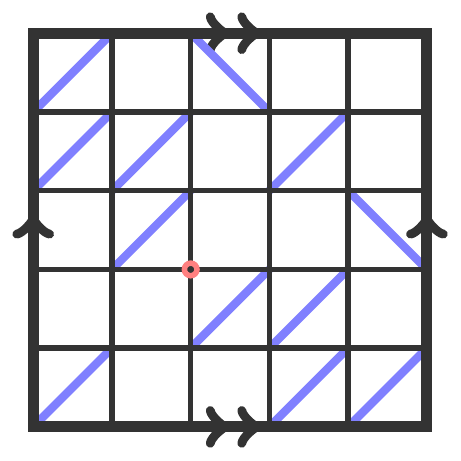
\begin{tikzpicture}
    \draw[black!80, line width=4, ->] (0,1)--(0,2.7);
    \draw[black!80, line width=4, ->] (5,1)--(5,2.7);
    \draw[black!80, line width=4, ->] (1,5)--(2.5,5);
    \draw[black!80, line width=4, ->] (1,5)--(2.9,5);
    \draw[black!80, line width=4, ->] (1,0)--(2.5,0);
    \draw[black!80, line width=4, ->] (1,0)--(2.9,0);

    \draw[blue!50, line width=3]
      (0,0)--(1,1) (0,3)--(1,4) (0,4)--(1,5)
      (1,2)--(2,3) (1,3)--(2,4)
      (2,1)--(3,2) (2,5)--(3,4)
      (3,0)--(4,1) (3,1)--(4,2) (3,3)--(4,4)
      (4,0)--(5,1) (4,3)--(5,2);
    \draw[black!80, line width=2] (0,0) grid (5,5);
    \draw[black!80, line width=4] (0,0) rectangle (5,5);

    \draw[red!50, line width=2] (2,2) circle (0.08);
  \end{tikzpicture}
  \caption{
    A maximal configuration of a $5 \times 5$ toroidal grid: $12$ diagonal lines
    can be drawn. The unused vertex is marked with a circle.
  }
\end{figure}
\begin{question}
  What is the greatest number of diagonals that can be drawn on a $n \times n$
  toroidal grid?
\end{question}

\begin{note}
  Let $m(n)$ be the maximum number of diagonals on an $n \times n$, grid.\\
  Then \begin{alignat*}{2}
  & m(2n) &&= 2n^2 \text{ and}\\
  2n^2 + n \leq\ & m(2n + 1) &&\leq 2n^2 + 2n.
\end{alignat*}
\end{note}

\begin{related}
  \item How many configurations exist for a given grid size up to group action?
  \item What if this is done on an $n \times m$ grid?
  \item What if this is done on a cylinder, Klein bottle, projective space, etc?
  \item What is the maximum number of diagonals that can go SW to NE?
  \item Does this generalize to three or more dimensions?
  \item Can something similar be done on a hexagonal or triangular grid?
  \item How many configurations exist if touching is allowed, but cycles aren't?
  \item What if we color edges of the grid rather than diagonals on the faces?
\end{related}

\begin{references}
  \item \url{https://oeis.org/A264041}
  \item \url{https://www.chiark.greenend.org.uk/~sgtatham/puzzles/js/slant.html}
\end{references}
\end{document}
